\documentclass[10pt,twocolumn]{article}
\usepackage[letterpaper,margin=0.75in,columnsep=0.25in]{geometry}
\usepackage[T1]{fontenc}
\usepackage{lmodern,microtype,amsmath,amssymb,booktabs,graphicx}
\usepackage[font=small,labelfont=bf]{caption}
\usepackage[numbers,sort&compress]{natbib}
\renewcommand{\bibfont}{\small}
\setlength{\bibsep}{2pt}
\usepackage{tikz}
\usetikzlibrary{arrows.meta,positioning}
\usepackage{xurl}
\usepackage[hidelinks]{hyperref}
\usepackage{placeins}
% Generated from saved artifacts by scripts/paper_assets.py.
\newcommand{\NItems}{500}
\newcommand{\NAtenModels}{6}
\newcommand{\NLfourModels}{4}
\newcommand{\NSamples}{10}
\newcommand{\AtenCount}{58,800}
\newcommand{\LfourCount}{12,000}
\newcommand{\TotalCount}{70,800}
\newcommand{\TimingCount}{10,800}
\newcommand{\TextRounded}{2--5\%}
\newcommand{\TextExact}{2.0\%--4.6\%}
\newcommand{\ThroughputLoss}{32--60\%}
\newcommand{\TokenRatioRange}{0.400--0.678}
\newcommand{\RootSeed}{20261101}
\newcommand{\BFCLVersion}{2026.3.23}
\newcommand{\MaxTokens}{512}
\newcommand{\ContextLimit}{8192}
\newcommand{\SampleTemperature}{0.7}
\newcommand{\TimingItems}{100}
\newcommand{\TimingRepetitions}{3}
\newcommand{\BootstrapCount}{5,000}
\newcommand{\OuterCount}{500}
\newcommand{\InnerCount}{1,000}
\newcommand{\OneItemGap}{0.2}
\newcommand{\PairedHalfWidth}{3}
\newcommand{\PairedEndpoint}{3.2}
\newcommand{\ItemsLlama}{834}
\newcommand{\MDDLlama}{3.87}
\newcommand{\ItemsQwen}{1,100}
\newcommand{\MDDQwen}{4.45}
\newcommand{\ItemRangeRounded}{800--1,100}
\newcommand{\TargetGap}{3}
\newcommand{\FollowupGross}{2.7296}
\newcommand{\FollowupEstimate}{3.1575}
\newcommand{\ProjectEstimate}{10.7213}
\newcommand{\FollowupForecast}{3.6089}
\newcommand{\TruncationsAten}{17}
\newcommand{\TruncationsLfour}{0}
\newcommand{\SyntaxFailuresAten}{913}
\newcommand{\ZeroUpper}{0.76\%}

\newcommand{\code}[1]{\texttt{#1}}
\setlength{\parindent}{1em}
\setlength{\parskip}{1pt}
\setlength{\textfloatsep}{10pt}
\setlength{\floatsep}{8pt}
\title{Leaderboard Noise: Greedy Variation Across Batches and Runs,\\One-Item Leads, and Their Mitigation}
\author{Mohith\\\small Chinmaya Vishwa Vidyapeeth, Kerala, India\\\small \texttt{achumohith14@gmail.com}}
\date{October 2026}
\begin{document}
\maketitle
\begin{abstract}
Default decoding changed about \TextRounded{} of greedy answers across batch settings. Same-batch repeats also varied, so this measures batch-setting plus run-to-run variation under default decoding. For Llama-3.2-3B and Qwen3-4B, each untied lead is one correct answer out of \NItems{} items; the reversal is a two-answer net swing. Each lead is a \OneItemGap{}-percentage-point margin inside exploratory paired intervals of roughly $\pm\PairedHalfWidth{}$ points, with endpoints reaching $\pm\PairedEndpoint{}$; it does not establish population superiority. The default winner sequence reverses between recorded A10 and L4 setups. Batch-invariant decoding removed all observed text changes across batch settings and timing repeats and produced identical decoded outputs across GPU tiers for every replicated model. Enabling it can itself change the winner. Its measured A10 cost was \ThroughputLoss{} lower median token throughput. Separate sampling-based projections require approximately \ItemRangeRounded{} items, with \NSamples{} answers per item per model, to detect a \TargetGap{}-point gap. The contribution is a practical replication using official BFCL scoring, auditable cost accounting, executed-source snapshots, and a reusable CLI, not a new variance decomposition or determinism mechanism.
\end{abstract}

\section{Introduction}
A leaderboard difference can be smaller than the measurement choices that produced it. Default decoding changed about \TextRounded{} of answers across batch settings while checkpoint, question, prompt, and request seed stayed fixed. Same-batch repeats also varied, so this measures batch-setting plus run-to-run variation under default decoding. That need not change correctness, and changed correctness need not change a clear model ordering. For the near-tied Llama/Qwen pair, each untied lead is one answer out of \NItems{} questions; the reversal is a two-answer net swing. Each lead lies within exploratory paired intervals of approximately $\pm\PairedHalfWidth{}$ percentage points.

This distinction bounds the claim. A different winner on the same finite set is a real measurement outcome. It is not evidence that the underlying model capabilities have exchanged order. Reporting a winner without its margin, the shared item set, or the batch setting can make a fragile result look decisive. In particular, a bootstrap flip fraction is not a posterior probability that a model is intrinsically better.

The study combines a \NAtenModels{}-model A10 experiment and an L4 replication of two observed-close pairs. The latter comparisons were frozen before L4 execution. Every comparison uses the same \NItems{} Python single-turn BFCL questions and official abstract syntax tree (AST) scoring. Across both stages, \TotalCount{} outputs were scored; repeated timing outputs do not create additional independent questions.

There are three practical results. First, default greedy text differences reach \TextExact{} across batch settings in the recorded models and GPU tiers. Same-batch timing repeats also varied, so these differences combine batch-setting and run-to-run variation. Second, the Llama/Qwen winner at request batches 1 and 32 reverses between A10 and L4, while batch 8 is tied on both. The other close pair retains its full-set order. Third, the documented batch-invariance setting removes all observed changes across batch settings and timing repeats and gives identical cross-tier text for all replicated models, but with a measured A10 throughput penalty. It also changes some answers, so activating it can select a different winner at a fixed batch.

The reusable contribution is \code{evalnoise}: a binary per-item result schema, paired uncertainty and rank-stability summaries, and approximate minimum-detectable-difference (MDD) planning. The empirical contribution is an inexpensive measurement-and-mitigation replication with retained failures, source hashes, and explicit operating limits. No new inference, grading, or bootstrap run was performed to prepare this paper.

\section{Related work}
\paragraph{Evaluation uncertainty.}
\citet{madaan2024variance} quantify benchmark variance across checkpoints and initializations and discuss discrete versus continuous measurements. Those training comparisons differ from decoding a frozen checkpoint under different serving batches. \citet{miller2024errorbars} develops paired comparisons, question-population assumptions, and power analysis. \citet{wang2025noise} separates prediction and data noise and applies paired analysis across model pairs. These works establish the statistical basis of this project; neither a variance decomposition nor all-pairs analysis is claimed as novel here.

\paragraph{Inference reproducibility.}
\citet{he2025nondeterminism} explains batch-dependent reduction arithmetic and proposes batch-invariant computation. Deterministic individual kernels do not by themselves imply an output independent of the requests served alongside it. The pinned vLLM documentation exposes the mitigation used here \citep{vllm032}. \citet{yuan2025numerical} directly studies numerical reproducibility under changes in batch size and GPU configuration and proposes higher-precision computation. \citet{gond2026llm42} proposes a verify--rollback approach instead of requiring batch invariance throughout. This project implements neither of those alternative mitigations.

\paragraph{Outputs, scores, and rankings.}
\citet{atil2025hosted} distinguishes agreement in raw outputs from agreement in parsed answers under hosted deterministic settings. \citet{song2025greedy} compares greedy decoding and sampling and motivates examining more than one output. The present study adds a focused small-model BFCL replication: it follows text differences through the official checker to a paired rank comparison, then measures one available mitigation's cost. BFCL supplies the benchmark and AST method \citep{patil2025bfcl}; the unbiased pass@$k$ estimator follows \citet{chen2021code}.

\section{Setup and measurement}
\subsection{Models, selection, and items}
The A10 roster is Qwen2.5-1.5B-Instruct, Qwen2.5-3B-Instruct, Qwen3-1.7B, Llama-3.2-3B-Instruct, xLAM-2-3b-fc-r, and Qwen3-4B-Instruct-2507. Model names below abbreviate these fixed checkpoints; immutable revisions are in Appendix~\ref{app:settings}. This is an open-weight roster with differing licenses, not a claim that all models have unrestricted open-source licenses.

Published BFCL scores initially selected comparisons among Qwen3-1.7B, Llama3B, and xLAM. Their gaps did not remain close on the common-prompting subset. All model pairs were retained rather than replacing models or questions. Two A10 default-serial pairs were within the \TargetGap{}-point target: Qwen2.5-3B versus Qwen3-1.7B, and Llama3B versus Qwen3-4B. Their selection is exploratory on A10; both were selected before any L4 results.

The frozen subset contains \NItems{} Python single-turn questions from simple, multiple, parallel, and parallel-multiple BFCL categories. Official prompting-mode instructions and \code{bfcl-eval==\BFCLVersion} AST scoring determine correctness. This subset's mean is not the official overall BFCL score. The checker parses function calls; generated code is not executed. Questions and answers, item IDs, source hashes, and prompt hashes remain in the release artifacts.

\begin{figure*}[t]
\centering
\begin{tikzpicture}[node distance=3mm and 4mm, box/.style={draw,rounded corners=1pt,fill=black!4,align=center,font=\small,inner sep=4pt}, arr/.style={-{Latex[length=1.7mm]},thick}]
\node[box,text width=25mm] (items) {\NItems{} frozen BFCL items\\Python single-turn};
\node[box,text width=26mm,right=of items] (a10) {A10: \NAtenModels{} models\\sampling (default) + greedy};
\node[box,text width=30mm,right=of a10] (arms) {Greedy: default / invariant\\batches 1, 8, 32};
\node[box,text width=23mm,right=of arms] (score) {Official BFCL\\AST checker};
\node[box,text width=25mm,right=of score] (analysis) {Paired-item analysis\\text, score, ranks};
\node[box,text width=49mm,below=6mm of a10.south,anchor=north west,xshift=-14mm] (l4) {L4: two close pairs (\NLfourModels{} models)\\greedy only; same items and greedy settings};
\draw[arr] (items)--(a10);\draw[arr] (a10)--(arms);\draw[arr] (arms)--(score);\draw[arr] (score)--(analysis);
\draw[arr] (items.south)|-(l4.west);\draw[arr] (a10.south)--node[right,font=\scriptsize]{select before L4}(l4.north);
\draw[arr] (l4.east)-|(arms.south);
\end{tikzpicture}

\caption{Measurement design. The same frozen \NItems{} items and official AST checker support the A10 study and L4 replication. Greedy decoding uses default and batch-invariant arms at request batches 1, 8, and 32. Sampling uses only the A10 default arm, with request batches of 16 and ten completions per item. The two close comparisons are exploratory choices from A10 but fixed before L4 outcomes.}
\label{fig:method}
\end{figure*}

\subsection{Decoding and timing}
Both arms use vLLM \code{0.32.0}, bfloat16, eager execution, prefix caching disabled, and an engine limit of 64 sequences. The intervention changes offline request submission batches, not a production HTTP load generator. Checkpoints, rendered prompts, output limits, and request seeds match across arms. The invariant arm sets \code{VLLM\_BATCH\_INVARIANT=1}. Each process passes a five-request smoke gate before evaluation.

Greedy evaluation generates one answer per question per batch condition. A separate A10 sampling condition generates \NSamples{} completions per question at temperature \SampleTemperature{} using vLLM's \code{n} parameter. Those answers support pass@1 and unbiased pass@5 and pass@10, but do not increase the number of independent questions.

Throughput uses \TimingRepetitions{} matched repetitions of a fixed \TimingItems{}-item subset per model, arm, and batch condition. Arm order alternates across repetitions in fresh processes. The measured region includes generation, device synchronization, and output collection. Loading, smoke checks, and per-condition warmup are excluded from throughput and included in cost. Generated-token and completion counts are retained, and timing outputs are scored to detect fast failures. There is no repeated L4 throughput experiment. In the saved A10 timing repeats, Qwen3-4B changes decoded text and correctness on \code{parallel\_multiple\_37} at the same batch size. The primary greedy conditions run once each in a fixed order, so the study does not isolate a pure batch-size effect.

\subsection{Uncertainty and planning}
The item bootstrap samples question IDs and carries both models' outputs at all batch settings together. It preserves paired question difficulty and within-question dependence across conditions. It uses \BootstrapCount{} resamples. A strict full-set flip requires opposite strict orders at two batch settings on the actual subset. A paired-bootstrap batch-flip fraction instead counts how often such a flip occurs after changing the empirical question mix. Ties alone do not count as flips.

Outer percentile intervals for flip fractions use \OuterCount{} outer paired-item draws and \InnerCount{} inner draws per outer sample. They are \emph{exploratory and unadjusted}, as are all confidence intervals in this paper. Ranking is discontinuous at ties; finite inner simulation contributes variation. A collapsed $[0,0]$ interval can reflect absent empirical patterns and is not a guarantee of zero population flips. Separate Monte Carlo intervals in the saved results concern only simulation precision conditional on this dataset.

For stochastic pass@1, planning estimates between-item variance after correcting for finite-repeat sampling variation. In the notation of the implementation, with $N$ items and $m$ samples per model,
\begin{equation}
\begin{aligned}
\operatorname{MDD}(N,m)&\approx(z_{1-\alpha/2}+z_{\mathrm{power}})\,\cdot\\
&\quad\sqrt{(\hat\sigma_{\mathrm{item}}^2+\hat v_{\mathrm{sampling}}/m)/N}.
\end{aligned}
\end{equation}
These are normal-approximation planning estimates, not guarantees for another question population. The saved calculations use a two-sided 5\% test and 80\% power. Adding answers to the same questions can reduce sampling noise but cannot remove between-question variation.

\section{Results}
\subsection{A one-item lead changes direction}
Table~\ref{tab:winners} names the winner at every setting for the focal pair. Under default decoding, A10 favors Qwen at batch 1, ties at batch 8, and favors Llama at batch 32. L4 favors Llama, ties, then favors Qwen. Thus the existence of a strict flip repeats, but the actual default winner at each untied batch is reversed across tiers. Figure~\ref{fig:ranks} shows the corresponding counts. Each untied lead is one correct answer out of \NItems{}; the batch-1 to batch-32 reversal is a two-answer net swing.

\begin{table}[t]
\centering\small
\begin{tabular}{llccc}
\toprule
GPU & Arm & Batch 1 & Batch 8 & Batch 32 \\
\midrule
A10 & Default & Qwen & Tie & Llama \\
A10 & Invariant & Llama & Llama & Llama \\
L4 & Default & Llama & Tie & Qwen \\
L4 & Invariant & Llama & Llama & Llama \\
\bottomrule
\end{tabular}

\caption{Higher observed score for Llama3B versus Qwen3-4B. All cells refer to the same \NItems{} items. Invariant Llama scores 458 and Qwen scores 457 in every cell. The default untied leads are also one item. A named winner is not established population superiority.}
\label{tab:winners}
\end{table}

The A10 batch-1 difference, Llama minus Qwen, is $-0.2$ points with an exploratory paired 95\% interval of $[-3.2,2.8]$ points. At batch 32 it is $+0.2$, with $[-2.8,3.2]$. The L4 default differences are $+0.2,0,-0.2$ points. Their intervals likewise include zero (Appendix~\ref{app:intervals}). The observed lead is therefore an order-of-magnitude smaller than the paired uncertainty. A small empirical reversal is the result, rather than a statistically separated capability ranking.

Qwen3-1.7B remains above Qwen2.5-3B at every default batch on both tiers. This null full-set flip result is retained. A nonzero bootstrap flip fraction can coexist with that stable observed order because resampling changes which questions receive weight.

\begin{figure*}[t]
\centering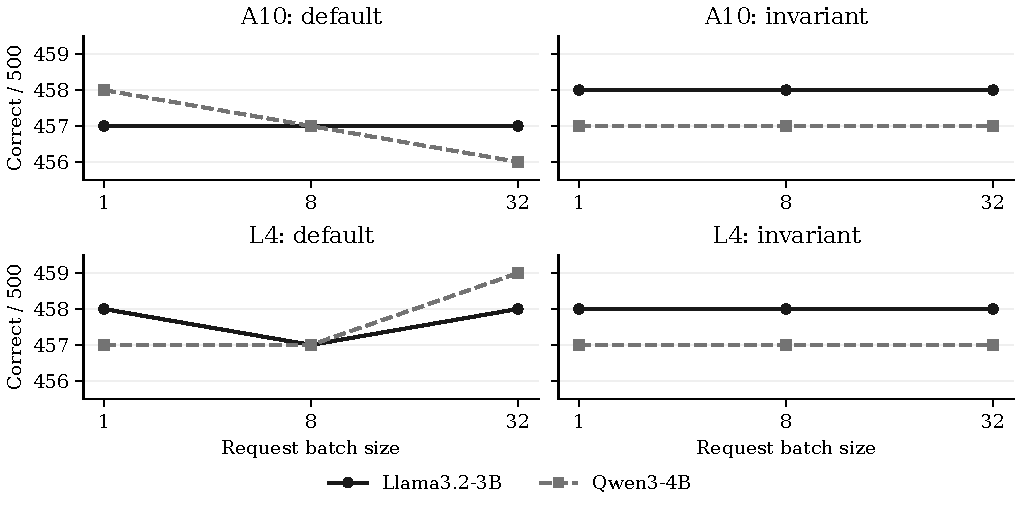
\includegraphics[width=0.93\textwidth]{figures/rank-order.pdf}
\caption{Focal-pair correct counts on A10 and L4, with default and invariant decoding. \textbf{The y-axis is zoomed to 455.5--459.5 correct calls out of \NItems{}}; one item is \OneItemGap{} percentage points. Line style and markers distinguish models in grayscale. These are fixed-set counts, not uncertainty intervals; exploratory paired intervals are reported separately.}
\label{fig:ranks}
\end{figure*}

\subsection{Text changes, mitigation, and its intervention effect}
Default greedy text differs across batch settings on \TextExact{} of questions, depending on the model and tier (Table~\ref{tab:changes}). Same-batch timing repeats also varied, so these counts measure batch-setting plus run-to-run variation under default decoding. These are decoded-text changes, not all correctness failures: the checker can accept different strings as the same valid call. Llama's A10 default text changes while its score remains constant across batches, illustrating why text, correctness, and rank require separate counts.

Invariant decoding has no observed text or correctness changes across the tested batch settings and timing repeats. For all \NLfourModels{} models replicated on L4, invariant decoded text and correctness also match A10 exactly at every batch setting. This equality is a result on the retained requests, not a theorem about other hardware or schedules.

Turning invariance on can itself change the winner. At A10 batch 1, default decoding favors Qwen, whereas invariant decoding favors Llama. At L4 batch 32 the setting has the same winner-changing effect. Invariance stabilizes the measurement under these batch changes; it does not preserve baseline answers or guarantee improved accuracy.

\begin{table*}[t]
\centering\small
\begin{tabular}{llrrrrc}
\toprule
GPU & Model & D text & D correct & I text & I correct & Expl. 95\% D text CI \\
\midrule
A10 & Qwen2.5-1.5B & 13 (2.6\%) & 4 & 0 & 0 & [1.53, 4.40] \\
A10 & Qwen2.5-3B & 18 (3.6\%) & 6 & 0 & 0 & [2.29, 5.62] \\
A10 & Qwen3-1.7B & 13 (2.6\%) & 6 & 0 & 0 & [1.53, 4.40] \\
A10 & Llama3.2-3B & 10 (2.0\%) & 0 & 0 & 0 & [1.09, 3.64] \\
A10 & xLAM2-3B & 20 (4.0\%) & 4 & 0 & 0 & [2.60, 6.10] \\
A10 & Qwen3-4B & 11 (2.2\%) & 5 & 0 & 0 & [1.23, 3.90] \\
L4 & Llama3.2-3B & 12 (2.4\%) & 2 & 0 & 0 & [1.38, 4.15] \\
L4 & Qwen3-4B & 12 (2.4\%) & 5 & 0 & 0 & [1.38, 4.15] \\
L4 & Qwen2.5-3B & 23 (4.6\%) & 8 & 0 & 0 & [3.08, 6.81] \\
L4 & Qwen3-1.7B & 12 (2.4\%) & 4 & 0 & 0 & [1.38, 4.15] \\
\bottomrule
\end{tabular}

\caption{Items with changed decoded text or correctness across batches, out of \NItems{} per row. D and I denote default and invariant arms. Default text-change intervals are \textbf{exploratory, unadjusted Wilson 95\% intervals}, in percent. Every invariant text count is zero; its exploratory interval is $[0,\ZeroUpper]$. Rows repeat the same questions and cannot be pooled as independent observations.}
\label{tab:changes}
\end{table*}

\subsection{Bootstrap rank stability}
Default bootstrap flip fractions are reported in Table~\ref{tab:flips}. The focal pair's L4 estimate is larger than its A10 estimate, but these intervals are broad and overlapping. The study does not claim a statistically separated hardware effect on flip probability. For invariant decoding both pairs have zero estimated flip fractions and collapsed outer intervals on both tiers. The empirical absence of relevant differing outcomes explains that collapse; it is not universal certainty.

\begin{table}[t]
\centering\scriptsize
\begin{tabular}{llrr}
\toprule
Pair & GPU & Flip (\%) & Expl. 95\% CI \\
\midrule
Llama / Qwen3-4B & A10 & 8.94 & [0.50, 23.66] \\
Llama / Qwen3-4B & L4 & 10.28 & [1.10, 27.81] \\
Qwen2.5-3B / Qwen3-1.7B & A10 & 13.18 & [0.60, 35.80] \\
Qwen2.5-3B / Qwen3-1.7B & L4 & 8.48 & [0.70, 28.45] \\
\bottomrule
\end{tabular}

\caption{Default paired-item bootstrap batch-flip fractions and \textbf{exploratory, unadjusted 95\% outer intervals}. Invariant fractions and outer intervals are zero for both pairs on both tiers, with the boundary limitation described in the text.}
\label{tab:flips}
\end{table}

\subsection{Throughput cost and evaluation size}
Across the A10 configurations, invariant/default median token-rate ratios range from \TokenRatioRange{}, or \ThroughputLoss{} lower throughput. Figure~\ref{fig:throughput} shows the median and observed range of the matched repetitions. These ranges are not confidence intervals. Completion rates are retained separately because changing outputs can change their lengths. No limiter profile or production tuning study was performed; these are measured configuration costs, not universal performance recommendations.

\begin{figure*}[t]
\centering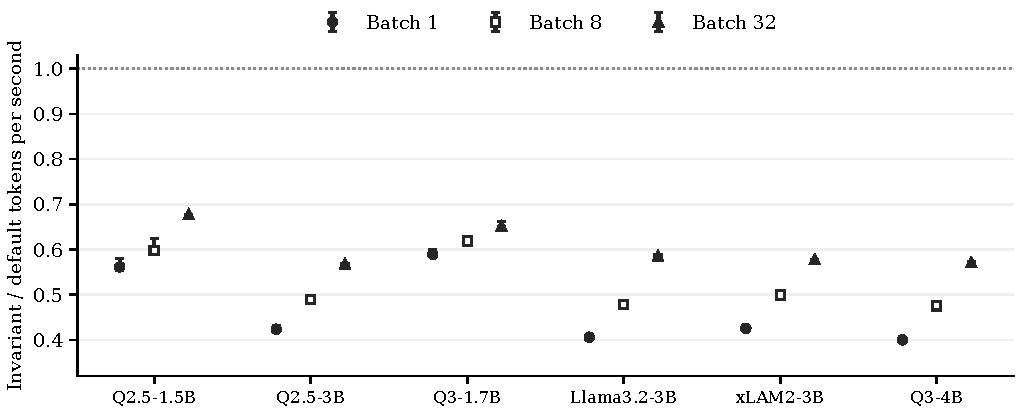
\includegraphics[width=0.93\textwidth]{figures/throughput.pdf}
\caption{A10 invariant/default generated-token throughput ratios. Markers distinguish request batches in grayscale. Points are medians and bars are observed ranges across \TimingRepetitions{} matched repetitions on \TimingItems{} items, \textbf{not confidence intervals}. The dotted line is equal throughput. No repeated L4 throughput measurement is claimed.}
\label{fig:throughput}
\end{figure*}

Table~\ref{tab:mdd} gives the saved stochastic pass@1 planning results. At \NItems{} items and \NSamples{} answers per item per model, approximate MDDs exceed the \TargetGap{}-point target. Required item counts are \ItemsLlama{} and \ItemsQwen{}, roughly \ItemRangeRounded{}. These projections use the paired variance of these two comparisons. They do not establish a universal sample-size threshold, and are not planning estimates for a one-answer greedy experiment. Under these estimates, increasing samples alone at the current item count cannot reach the target gap.

\begin{table}[t]
\centering\scriptsize
\begin{tabular}{lrr}
\toprule
Pair & MDD (pp) & Items needed \\
\midrule
Llama / Qwen3-4B & 3.87 & 834 \\
Qwen2.5-3B / Qwen3-1.7B & 4.45 & 1,100 \\
\bottomrule
\end{tabular}

\caption{Exploratory A10 sampling-based planning: current MDD at \NItems{} items and \NSamples{} samples, and items needed for a \TargetGap{}-point gap at the same samples per model. Estimates assume a two-sided 5\% test and 80\% power.}
\label{tab:mdd}
\end{table}

\subsection{Cost accounting and retained failures}
The L4 follow-up's original forecast was \$\FollowupForecast{}. Across both L4 allocations, provisional app-specific gross metering was \$\FollowupGross{}, and the conservative estimate was \$\FollowupEstimate{}. The full project estimate, including the A10 study, pilot, and setup failures, was \$\ProjectEstimate{}. Invoice actuals remain unknown; credit offsets and unrelated project usage do not reduce the recorded gross costs.

A10 recovery preserved the completed anchor and continued the other models on another card. L4 was preempted after the focal pair finished; only the unfinished pair resumed. Completed checkpoints and their scored rows were preserved. Unretained partial execution is charged but not scored or imputed. The accounting excludes GPU queue waiting after preemption and distinguishes allowances from spend. All owned study apps were stopped, reservations released, and temporary result volumes deleted after verified downloads. No new remote work was launched for this manuscript.

\section{Limitations}
\paragraph{A small empirical flip.}
Each decisive observed lead is one item and its reversal is a two-answer net swing, while paired uncertainty is approximately $\pm\PairedHalfWidth{}$ points. There is one frozen subset and no independent new question sample. The conclusion is sensitivity of the recorded rank, not that GPU or batch choice reliably changes an unseen-population winner. Items sharing function templates can violate independent-item assumptions. All intervals are exploratory and unadjusted; collapsed intervals do not rule out unobserved patterns.

\paragraph{Hardware is not isolated.}
Every requested pair shares one physical card per tier, but there is no randomized crossover over many cards. CPU caps and hosting allocations differ, and generation history differs: A10 default sampling precedes greedy evaluation, whereas L4 starts greedy evaluation after smoke and warmup. The retained drivers all record \code{610.57.04}; the evidence does not support calling their version strings different. Host identities are not uniformly captured, and load observations are not a controlled host study. GPU architecture is therefore not causally isolated. Appendix~\ref{app:settings} discloses the available hardware and execution metadata.

\paragraph{Scope of the evaluation.}
This is a single-turn Python BFCL subset under common prompting, not the full leaderboard or a native-tool API benchmark. Training-seed, prompt, hosted-provider drift, and executed-code variation are not measured. Comparisons found close on A10 remain exploratory there. The L4 repetition tests those selected comparisons and does not turn the A10 selection into an independently selected experiment. Timing repetitions support within-configuration ranges only.

\paragraph{Source attestation.}
Executed-source snapshots and hashes are shipped, including the before/after Llama beginning-of-sequence (BOS) correction. Earlier A10 processes recorded launch hashes but not runtime worker self-hashes; later A10 and L4 workers recorded self-hashes. That distinction is explicit in \code{provenance/manifest.json}. Snapshots make changes reviewable; they are not independent cryptographic attestations of an entire execution environment.

\section{Conclusion}
Default decoding changed about \TextRounded{} of greedy answers across batch settings. Same-batch repeats also varied, so this measures batch-setting plus run-to-run variation under default decoding. Each untied lead for the near-tied pair is one correct answer out of \NItems{}; the reversal is a two-answer net swing. The default ordering reverses between the recorded A10 and L4 setups. The margin remains within broad paired uncertainty. Batch invariance removed all observed changes across batch settings and timing repeats and matched outputs across tiers, at an A10 throughput cost, while sometimes changing the winner itself. A useful evaluation report should therefore fix or disclose batch policy, repeat default runs, retain per-item outcomes, show paired uncertainty, and distinguish stable text from a separated score difference.

\section{Data and code availability}
The public study repository is \url{https://github.com/mohi-devhub/leaderboard-noise}. The paper and reproducibility archive are available in release \code{v0.1.0-paper} at \url{https://github.com/mohi-devhub/leaderboard-noise/releases/tag/v0.1.0-paper}. The archive contains the saved per-item artifacts, pinned environment definitions, official-checker references, CLI, manuscript sources, vector figures, \code{provenance/} snapshots, and SHA256 checksums. Every empirical table and plot is generated from saved summaries; \code{paper/artifact-map.json} maps values to their inputs.

Original project code is MIT-licensed. BFCL-derived data and attribution retain Apache-2.0 in \code{third\_party/BFCL/}; the Python distributions and release archive include both license texts and the BFCL notice. Qwen2.5-3B has research/noncommercial terms, xLAM uses CC BY-NC 4.0, and Llama requires its community license and acceptable-use policy. Model weights are not redistributed.

\bibliographystyle{plainnat}
\bibliography{references}
\clearpage
\appendix
\onecolumn
\section{Complete settings and execution disclosure}\label{app:settings}
\paragraph{Frozen inputs.}
The subset is \code{BFCL\_v4\_python\_ast\_subset}, with \BFCLVersion{} of the official evaluation package. It contains 200 simple-Python, 100 multiple, 100 parallel, and 100 parallel-multiple items, sampled with \code{stdlib Random.sample} under seed \RootSeed{}. The exact IDs and source/question/answer SHA256 hashes are in \code{experiments/subset.json}. Model revisions and item/prompt definitions were frozen before their respective execution. The three original published-score comparisons were fixed before A10 execution; the two observed-close pairs were fixed before L4 execution.

\paragraph{Serving and tokenization.}
vLLM \code{0.32.0}, Python \code{3.12.12}, PyTorch \code{2.13.0}, CUDA runtime \code{13.0}, transformers \code{5.19.0}, and tokenizers \code{0.23.3} are retained in inference metadata. Weights and tokenizer use the same pinned revision, \code{trust\_remote\_code=False}, and safetensors loading. Dtype is bfloat16, tensor parallelism is one, eager execution is on, prefix caching is off, GPU-memory utilization is 0.85, maximum context is \ContextLimit{}, and the generation cap is \MaxTokens{} tokens. Engine concurrency is fixed at 64. Default sets the invariance environment variable to zero and the mitigation sets it to one before vLLM import.

Greedy request batches are 1, 8, and 32 with temperature zero and one sample. Sampling uses temperature \SampleTemperature{}, top-$p=1$, \NSamples{} child samples, and request batches of 16. Qwen3-1.7B passes \code{enable\_thinking=False} in chat-template arguments. Qwen3-4B-Instruct-2507 uses its fixed checkpoint's template. Llama rendered chats already contain BOS, so \code{add\_special\_tokens=False} is applied to benchmark and warmup prompts before Llama begins. Other models retain their defaults; preflight token IDs were unchanged for their frozen prompts.

\paragraph{Seeds.}
The engine and smoke seed is \RootSeed{}. Per-question sampling seeds use
\[
 s_{m,i}=\RootSeed{}+10^6\,j_m+100\,i,
\]
where $j_m$ is the frozen model index and $i$ the frozen item index. Per-request parameter objects avoid broadcasting one seed stream across unrelated prompts. The formula and its source snapshots are shipped; child-sample independence remains a statistical assumption. The outer/inner flip seeds and all condition-specific analysis seeds are retained in JSON, rather than inferred from a single root seed.

\paragraph{Analysis.}
Item uncertainty uses \BootstrapCount{} paired resamples. Flip outer intervals use \OuterCount{} outer and \InnerCount{} inner draws. Tie handling is strict and explicit. Wilson text-change and Monte Carlo precision intervals, percentile item and outer intervals, and all paired gap intervals are exploratory and unadjusted. Stochastic pass@1 averages per-item success rates. For $c$ correct generations among $n$, the unbiased estimator is $1-\binom{n-c}{k}/\binom{n}{k}$ with $n\ge k$, following \citet{chen2021code}. It requires independent, identically distributed generations and a way to recognize correctness. Conditional within-item pass@$k$ resampling for $k>1$ is diagnostic because finite-repeat bias can be substantial; it is not pooled with item uncertainty. Variance clipping and unidentifiable components are flagged by the CLI.

\begin{table}[htbp]\centering\small
\begin{tabular}{lllr}
\toprule
Pair & GPU & Arm & Flip-analysis seed \\
\midrule
Llama3.2-3B / Qwen3-4B & A10 & default & 20261232 \\
Llama3.2-3B / Qwen3-4B & A10 & batch\_invariant & 20261233 \\
Llama3.2-3B / Qwen3-4B & L4 & default & 20261201 \\
Llama3.2-3B / Qwen3-4B & L4 & batch\_invariant & 20261202 \\
Qwen2.5-3B / Qwen3-1.7B & A10 & default & 20261152 \\
Qwen2.5-3B / Qwen3-1.7B & A10 & batch\_invariant & 20261153 \\
Qwen2.5-3B / Qwen3-1.7B & L4 & default & 20261211 \\
Qwen2.5-3B / Qwen3-1.7B & L4 & batch\_invariant & 20261212 \\
\bottomrule
\end{tabular}

\caption{Saved paired-flip analysis seeds. Each seeds the stated paired resampling procedure; outer and inner counts remain \OuterCount{} and \InnerCount{}. Condition-specific item/sampling analyses retain the root seed in their JSON.}
\end{table}

\paragraph{Timing and resources.}
A10 workers request two and cap four CPU cores; L4 workers request and cap two. RAM requests are 8 GiB with a 16 GiB cap. The process-visible CPU count and load observations are stored with each model. Five smoke requests generate at most eight tokens each. Each evaluated batch setting warms on its first request batch before device synchronization and timing. A10 throughput uses \TimingRepetitions{} fresh-process repetitions of \TimingItems{} fixed items per arm and batch, with default-first, invariant-first, default-first arm ordering. Repetition zero also contains the primary conditions. The L4 arms collect greedy primary rows only. No L4 timing ratio is inferred from end-to-end job duration.

\begin{table}[t]\centering\scriptsize
\begin{tabular}{lrlp{2.1cm}}
\toprule
Model & Seed index & Immutable revision & License \\
\midrule
Qwen2.5-1.5B & 1 & \texttt{989aa7980e4cf806f80c7fef2b1adb7bc71aa306} & apache-2.0 \\
Qwen2.5-3B & 11 & \texttt{aa8e72537993ba99e69dfaafa59ed015b17504d1} & other \\
Qwen3-1.7B & 12 & \texttt{70d244cc86ccca08cf5af4e1e306ecf908b1ad5e} & apache-2.0 \\
Llama3.2-3B & 13 & \texttt{0cb88a4f764b7a12671c53f0838cd831a0843b95} & llama3.2 \\
xLAM2-3B & 14 & \texttt{be83286f6a1a82c8bd4bfb751190271f58693f30} & cc-by-nc-4.0 \\
Qwen3-4B & 15 & \texttt{cdbee75f17c01a7cc42f958dc650907174af0554} & apache-2.0 \\
\bottomrule
\end{tabular}

\caption{Frozen model revisions and seed indices. License metadata is an identifier, not a replacement for the linked official license terms in the release artifacts. No weights are included.}
\end{table}
\begin{table}[t]\centering\scriptsize
\begin{tabular}{llllr}
\toprule
GPU & Model & Driver & UUID prefix & Visible host CPUs \\
\midrule
A10 & Qwen2.5-1.5B & 610.57.04 & \texttt{df755a7a} & 4 \\
A10 & Qwen2.5-3B & 610.57.04 & \texttt{2c28e71d} & 4 \\
A10 & Qwen3-1.7B & 610.57.04 & \texttt{2c28e71d} & 4 \\
A10 & Llama3.2-3B & 610.57.04 & \texttt{2c28e71d} & 4 \\
A10 & xLAM2-3B & 610.57.04 & \texttt{2c28e71d} & 4 \\
A10 & Qwen3-4B & 610.57.04 & \texttt{2c28e71d} & 4 \\
L4 & Llama3.2-3B & 610.57.04 & \texttt{839082a9} & 2 \\
L4 & Qwen3-4B & 610.57.04 & \texttt{839082a9} & 2 \\
L4 & Qwen2.5-3B & 610.57.04 & \texttt{5d989e6c} & 2 \\
L4 & Qwen3-1.7B & 610.57.04 & \texttt{5d989e6c} & 2 \\
\bottomrule
\end{tabular}

\caption{Recorded physical assignment and driver versions. Full UUIDs, host-load observations, package versions, CPU limits, and source attestations are available in \code{paper/artifact-map.json} and original model JSON. Visible CPUs are observations, not a claim of equal effective host capacity.}
\end{table}

\paragraph{Source history.}
The initial A10 worker and the before-BOS worker share the recorded launch hash. The corrected worker adds Llama-specific tokenization handling and runtime self-hashing; L4 adds greedy-only controls without changing matched per-item seeds or inference settings. The runtime correction was installed before Llama's first generation. Captured serialized A10 GPU/controller function bodies and original L4 launch sources are copied byte for byte into \code{provenance/}. Its manifest names the frozen source path, recorded hash, attestation type, affected processes, and copied hash. Earlier A10 workers lack runtime self-hashes and are marked launch-attested. The packaging check rejects missing or mismatched source bytes.

\paragraph{Security and recovery.}
The images use official hash-locked dependencies, pinned compiler packages, a CPU compiler preflight, and package audits with documented user-approved setuptools applicability exceptions. An audit with those exceptions means zero unaccepted findings, not zero published advisories. Secrets are excluded from result artifacts and package inputs. The CPU AST checker parses outputs; it does not execute generated functions. Detached jobs checkpoint per model. After L4 preemption, a committed execution claim blocks regenerated outputs on platform replay. The CPU controller's nonpreemptible resource multiplier is included in accounting; it does not make the GPU nonpreemptible.

\FloatBarrier
\section{Exploratory paired intervals and sampling results}\label{app:intervals}
The following intervals are exploratory and unadjusted. All gaps are model A minus model B in percentage points. They show the scale of uncertainty surrounding the one-item observed leads; none establishes a separated population winner for the focal pair.
\begin{table}[h]\centering\scriptsize
\begin{tabular}{lllrrr}
\toprule
Pair & GPU & Arm & Batch & Gap (pp) & Expl. 95\% CI (pp) \\
\midrule
Llama3.2-3B minus Qwen3-4B & A10 & default & 1 & -0.20 & [-3.20, 2.80] \\
Llama3.2-3B minus Qwen3-4B & A10 & default & 8 & +0.00 & [-3.00, 3.00] \\
Llama3.2-3B minus Qwen3-4B & A10 & default & 32 & +0.20 & [-2.80, 3.20] \\
Llama3.2-3B minus Qwen3-4B & A10 & batch\_invariant & 1 & +0.20 & [-2.80, 3.20] \\
Llama3.2-3B minus Qwen3-4B & A10 & batch\_invariant & 8 & +0.20 & [-2.80, 3.20] \\
Llama3.2-3B minus Qwen3-4B & A10 & batch\_invariant & 32 & +0.20 & [-2.80, 3.20] \\
Llama3.2-3B minus Qwen3-4B & L4 & default & 1 & +0.20 & [-2.80, 3.20] \\
Llama3.2-3B minus Qwen3-4B & L4 & default & 8 & +0.00 & [-3.00, 3.00] \\
Llama3.2-3B minus Qwen3-4B & L4 & default & 32 & -0.20 & [-3.00, 2.80] \\
Llama3.2-3B minus Qwen3-4B & L4 & batch\_invariant & 1 & +0.20 & [-2.80, 3.20] \\
Llama3.2-3B minus Qwen3-4B & L4 & batch\_invariant & 8 & +0.20 & [-2.80, 3.20] \\
Llama3.2-3B minus Qwen3-4B & L4 & batch\_invariant & 32 & +0.20 & [-2.80, 3.20] \\
Qwen2.5-3B minus Qwen3-1.7B & A10 & default & 1 & -1.60 & [-5.20, 1.80] \\
Qwen2.5-3B minus Qwen3-1.7B & A10 & default & 8 & -0.80 & [-4.20, 2.60] \\
Qwen2.5-3B minus Qwen3-1.7B & A10 & default & 32 & -1.20 & [-4.80, 2.20] \\
Qwen2.5-3B minus Qwen3-1.7B & A10 & batch\_invariant & 1 & -2.00 & [-5.60, 1.60] \\
Qwen2.5-3B minus Qwen3-1.7B & A10 & batch\_invariant & 8 & -2.00 & [-5.60, 1.60] \\
Qwen2.5-3B minus Qwen3-1.7B & A10 & batch\_invariant & 32 & -2.00 & [-5.60, 1.60] \\
Qwen2.5-3B minus Qwen3-1.7B & L4 & default & 1 & -1.00 & [-4.40, 2.40] \\
Qwen2.5-3B minus Qwen3-1.7B & L4 & default & 8 & -1.00 & [-4.60, 2.40] \\
Qwen2.5-3B minus Qwen3-1.7B & L4 & default & 32 & -1.20 & [-4.60, 2.20] \\
Qwen2.5-3B minus Qwen3-1.7B & L4 & batch\_invariant & 1 & -2.00 & [-5.60, 1.60] \\
Qwen2.5-3B minus Qwen3-1.7B & L4 & batch\_invariant & 8 & -2.00 & [-5.60, 1.60] \\
Qwen2.5-3B minus Qwen3-1.7B & L4 & batch\_invariant & 32 & -2.00 & [-5.60, 1.60] \\
\bottomrule
\end{tabular}

\caption{Saved exploratory 95\% paired item-bootstrap gap intervals. No intervals were recomputed for this manuscript.}
\end{table}
\begin{table}[t]\centering\small
\begin{tabular}{lrrrr}
\toprule
Model & pass@1 (\%) & Expl. 95\% CI & pass@5 & pass@10 \\
\midrule
Qwen2.5-1.5B & 79.36 & [76.36, 82.30] & 88.76 & 91.00 \\
Qwen2.5-3B & 83.58 & [80.56, 86.48] & 89.33 & 91.00 \\
Qwen3-1.7B & 86.48 & [83.72, 89.16] & 89.55 & 90.00 \\
Llama3.2-3B & 89.12 & [86.78, 91.32] & 94.08 & 95.20 \\
xLAM2-3B & 74.50 & [71.32, 77.70] & 84.32 & 87.40 \\
Qwen3-4B & 91.30 & [88.94, 93.50] & 94.03 & 95.20 \\
\bottomrule
\end{tabular}

\caption{Saved A10 sampling scores. pass@1 intervals are exploratory 95\% item-bootstrap intervals; pass@5 and pass@10 point estimates use the unbiased estimator. Timing repetitions and L4 greedy outputs do not add independent sampling observations.}
\end{table}

\FloatBarrier
\section{Reproduction and release contents}
The paper build renders tables and vector figures from frozen JSON using \code{scripts/paper\_assets.py}, then compiles \code{paper/main.tex}. It performs no inference, checker rerun, or bootstrap simulation. \code{paper/artifact-map.json} records every input digest and the origin of numerical macros. The PDF builder and TeX toolchain hashes are pinned separately from the inference environment. The method diagram is vector TikZ. Both quantitative figures are vector PDF with grayscale line and marker distinctions.

The release packager includes the original MIT license, Apache-2.0 BFCL license and attribution notice, pinned source snapshots, data/configuration inputs, paper sources and PDF, verification receipts, and a per-file SHA256 manifest. It rejects secret/cache/weight paths and missing mandatory files. An external checksum authenticates the archive bytes relative to the recorded digest; it is not a third-party signature. The pre-release audit is retained in \code{AUDIT.md}, and its wording corrections are listed in \code{docs/REVISION\_SENTENCES.md}. Build and packaging scripts do not publish releases; publication follows verification.
\end{document}
